\chapter{Volumenberechnung mit der Kinect}
\section{Anforderungen und Ziele}
Um sich nicht mehr auf die Klassifizierung verschiedener Vordefinierter Gläsertypen verlassen zu müssen, soll der Weinschorle-Automat in der Lage sein das Volumen eines Glases mithilfe des Tiefensensors einer Microsoft Kinect zu berechnen.

\section{Vorgehen}
\subsection{Limitationen der Kinect}
Bevor wir die Kinect in den Weinschorle-Automaten einbezogen haben, testeten wir deren Möglichkeiten. Nach der Installation von notwendiger Treiber-Software begannen wir mit den Verschiedenen Modi der Kinect zu experimentieren.

Nach ersten Tests und Recherchen mussten wir feststellen, dass der Tiefensensor der Kinect bei Objekten näher als ca. 50cm keine zuverlässigen Werte liefern kann. Diese Tatsache schränkte die Positionierungsmöglichkeiten am Weinschorle-Automaten deutlich ein. Übrig blieben die beiden Möglichkeiten: 
\begin{enumerate}
	\item Vogelperspektive
	\item Frontalperspektive
\end{enumerate}

\subsection{Vogelperspektive}
Unsere erste Idee war es die Gläser von direkt über ihnen aufzunehmen. Dazu müssten wir allerdings einen Überbau konstruieren, um die Kinect mindestens 50cm über den Glasrändern anbringen zu können. (Abbildung \ref{fig:position_zur_vogelperspektive})
\begin{figure}
	\centering
	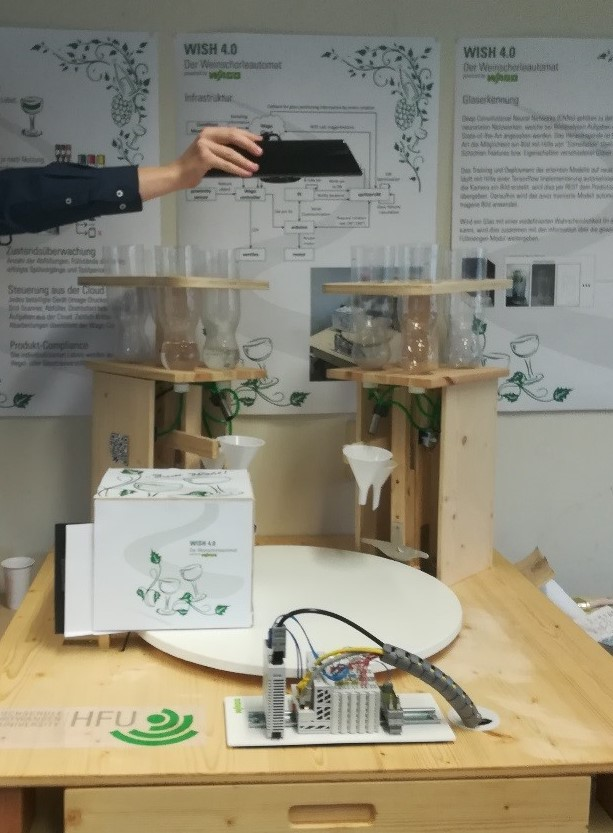
\includegraphics[width=0.5\linewidth]{content/pictures/position_zur_Vogelperspektive}
	\caption{Platzierung der Kinect für Vogelperspektive}
	\label{fig:position_zur_vogelperspektive}
\end{figure}
Vorteile dieser Positionierung sind zum einen die einfachere Messung des Volumens, da wir nur zwei Messpunkte im selben Bild benötigen. Einen für die Entfernung des Randes und einen für die Entfernung des Glasbodens zur Kinect. Daraus lässt sich dann einfach die Füllhöhe als Differenz der beiden werte berechnen. Mithilfe des Radius könnten wir das Volumen des Glases abschätzen. 

Zum andern könnten wir bei dieser Positionierung die RGB-Kamera der Kinect einsetzen, um beispielsweise die Sauberkeit des Drehtellers zu überprüfen (siehe Verschmutzung des Drehtellers).

Ein Nachteil wäre der zusätzliche Aufwand einen Überbau zu konstruieren, an dem wir die Kinect befestigen können. Außerdem muss bei diesem Ansatz das Glas zwischen den beiden Trichtern des Weinschorle-Automaten vermessen werden (siehe Abbildung \ref{fig:aufnahme_vogel}a). Dies würde uns dazu zwingen den Drehteller nach der Vermessung gegen den Uhrzeigersinn zu drehen. Da zu diesem Zeitpunkt bereits ein neues Glas auf dem Drehteller stehen könnte, würde dessen Füllroutine behindert. 

Zum Scheitern dieses Ansatzes führte schließlich die Untauglichkeit der Kinect für die Messung des Glasrandes, wie man in Abbildung \ref{fig:aufnahme_vogel}b erkennen kann. Im besten Fall sollte man an der Stelle des Glasrandes einen dunkel-grauen Ring erkennen können. Jedoch nimmt die Kinect nur undefinierte Werte auf (repräsentiert durch weiß im Bild) Die Kinect gibt Tiefenwerte von 0 (schwarz) bis 2048(weiß) für jeden Pixel in ihrem Tiefenbild an. 

\clearpage
\begin{figure}
	\centering
	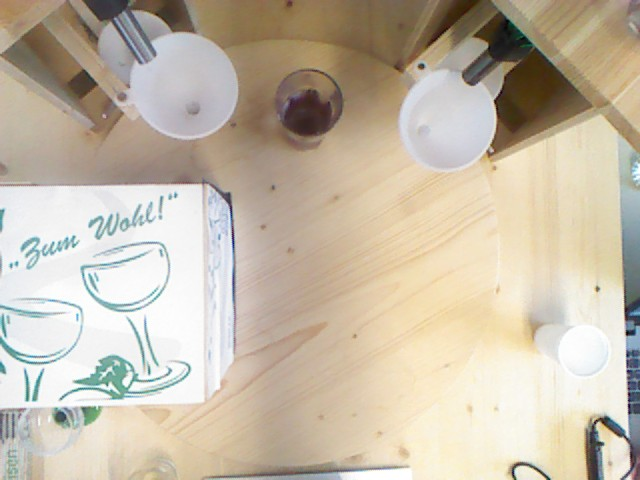
\includegraphics[width=0.45\linewidth]{content/pictures/vogel_rgb}
	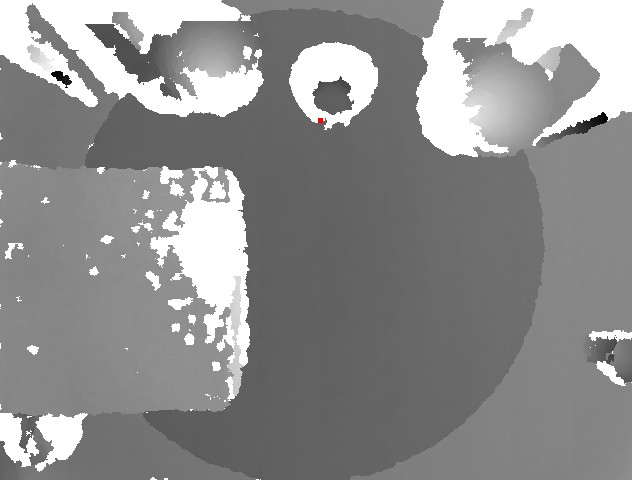
\includegraphics[width=0.45\linewidth]{content/pictures/vogel_depth}
	\caption{Kinect Aufnahme aus Vogelperspektive, RGB-Modus links (a), Tiefen-Modus rechts (b)}
	\label{fig:aufnahme_vogel}
\end{figure}

\subsection{Frontalperspektive}
Alternativ bliebe noch die Möglichkeit die Gläser frontal aufzunehmen, während sie unter dem ersten Trichter auf das Befüllen warten (siehe Abbildung \ref{fig:position_zur_frontalperspektive}a). Dazu positionieren wir die Kinect in der vorderen rechten Ecke des Tisches (siehe Abbildung \ref{fig:position_zur_frontalperspektive}b).
Aus dieser Positionierung ergeben sich folgende Vorteile:
\begin{itemize}
	\item Kein Überbau benötigt
	\item Keine Rotation des Drehtellers gegen den Uhrzeigersinn
\end{itemize}
Die Untauglichkeit der Kinect zuverlässige Werte zu liefern führt auch hier, ähnlich wie bei der Vogelperspektive, zum Scheitern des Ansatzes.

\begin{figure}[!h]
	\centering
	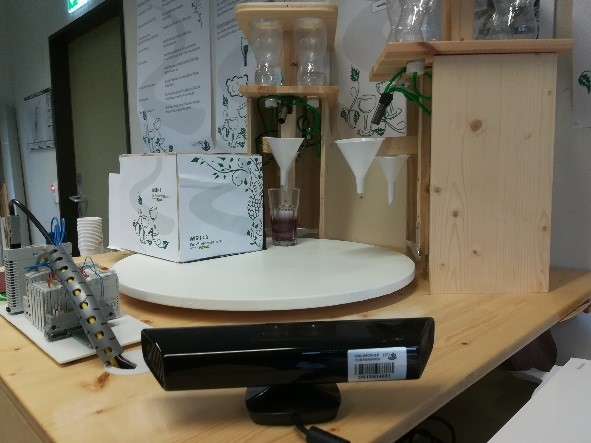
\includegraphics[width=0.45\linewidth]{content/pictures/position_zur_Frontalperspektive_behind}
	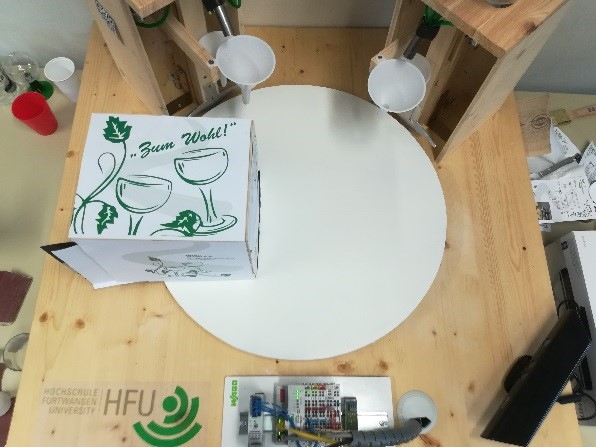
\includegraphics[width=0.45\linewidth]{content/pictures/position_zur_Frontalperspektive_top}
	\caption{Platzierung der Kinect für Frontalpositionierung}
	\label{fig:position_zur_frontalperspektive}
\end{figure}

\section{Fazit zur Kinect}
Die Kinect eignet sich nicht für Distanzen unter 50cm Entfernung, was schwer mit den Dimensionen des Weinschorle-Automaten zu vereinbaren ist. (z.B. mit einem Überbau). 

Weiterhin reicht die Auflösung der Tiefenkamera nicht aus um schmale Flächen wie einen Glas- oder Becherrand zu erfassen, was zum Scheitern unserer ersten Idee führte. 

Zuletzt scheitert diese Idee an der Tatsache, dass die Tiefenkamera der Kinect durch Projektionen von Infrarotlicht funktioniert, wobei aus den Reflektionen der Objekte ein Tiefenbild generiert wird. Durch fehlende Fähigkeit von Glas Licht zu reflektieren, ist es nahezu unmöglich dieses zu vermessen. 

Zusammenfassend genügen die Fähigkeiten der Kinect nicht den Anforderungen des Projektes.
